
\subsection{Waiting to Be Right}

He finally turned slightly, catching her reflection in the window glass.
“And the FX legs?”

“Still parked. Cross-asset logic isn’t tuned for New York latency. If the hedge legs fire early, we misprice the unwind.”

He gave the faintest nod.
“Chicago?”

“Still sandboxed,” she said. “The derivs desk are decoupled on their clock, and their book.”

David looked away from the window at last.
“So the framework’s stitched, but only London’s alive.”

Kayla nodded.
“We’re letting the aggregator read the book before it touches size.”

He watched her now, full-on.
“Good. Just make sure it doesn’t misread what it sees.”

But even as he said it, the words were already replaying in his mind —
not Kayla’s, but the voices from Zurich.
From the windowless ops room with a latency heatmap projected above the trading floor like a weather 
radar for execution risk.

On the whiteboard in Zurich, someone had drawn three boxes with a black marker — sharp, deliberate strokes labeled FX, Derivs, 
and Cash. They weren’t aligned. Not neatly. Not in a grid.
They floated, slightly off-axis, as if even the architecture was hedging its bets.

Beneath them, the arrows began — not just connectors, but arguments.

A thick, straight arrow ran from FX to Derivs, as if to say: this part we trust.

A dashed line linked Derivs to Cash, trailing off before it reached the box — hesitant, like a promise made under stress.

Then came the curved arrow, looping from Cash back toward FX, not directly, but arcing like it had been dragged there by uncertainty. Like it wanted to get there, but wasn’t convinced it should.

The lines weren’t just directional.
They were diagnostic.
They mapped not just flow, but doubt.

It wasn’t a process diagram.
It was a forecast of hesitation.

And David remembered thinking:
This wasn’t logic. This was latency rendered as belief.

\medskip

\begin{figure}[H]
    \centering
    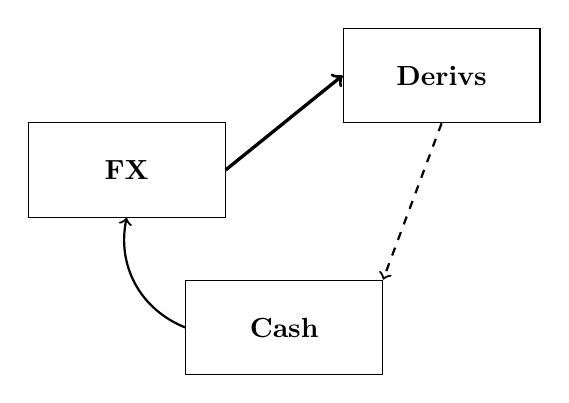
\begin{tikzpicture}[
      node distance=3cm,
      box/.style={draw, minimum width=2.5cm, minimum height=1.2cm, font=\bfseries, align=center},
      thickarrow/.style={->, line width=1.2pt},
      dashedarrow/.style={->, thick, dashed},
      curvedarrow/.style={->, thick, bend left=40}
    ]
    
    % Nodes
    \node[box] (fx) at (0,0) {FX};
    \node[box] (derivs) at (4,1.2) {Derivs};
    \node[box] (cash) at (2,-2) {Cash};
    
    % Arrows
    \draw[thickarrow] (fx.east) -- (derivs.west);
    \draw[dashedarrow] (derivs.south) -- (cash.north east);
    \draw[curvedarrow] (cash.west) to (fx.south);
    
    \end{tikzpicture}
    
    \vspace{1.5em}
    
    % Vertical Legend
    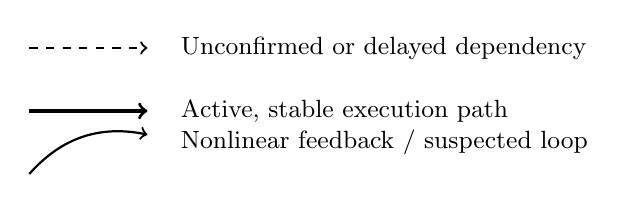
\begin{tikzpicture}[
      legend/.style={font=\small, anchor=west},
      dashsample/.style={->, thick, dashed},
      boldsample/.style={->, line width=1.2pt},
      curvesample/.style={->, thick, bend left=30}
    ]
    
    % Samples - vertical layout
    \draw[dashsample] (0,0) -- (1.5,0);
    \node[legend] at (1.8,0) {Unconfirmed or delayed dependency};
    
    \draw[boldsample] (0,-0.8) -- (1.5,-0.8);
    \node[legend] at (1.8,-0.8) {Active, stable execution path};
    
    \draw[curvesample] (0,-1.6) to (1.5,-1.1);
    \node[legend] at (1.8,-1.2) {Nonlinear feedback / suspected loop};
    
    \end{tikzpicture}
    
    \caption*{Legend: Arrow styles represent types of relationships between execution components.}
\end{figure}
    

\medskip

David had stood at the front and said:
“This is not a relay. It’s a choreography.”

“Then why not fire FX first?” someone had asked.
“Because FX moves before we do,” he replied. “If we hedge before the primary touches, we tell the 
street what we’re about to do.”

“And derivs?”

“They live in Chicago time. If we sync their clock to London, we break their book. If we don’t, 
we break ours.”

It had been one of those sessions — the kind where no one raised their voice because everyone 
understood the cost of being wrong.

What they had built wasn’t fragile, not exactly.
But it was threaded — stitched across markets like a pressure-sensitive suit.

Touch one panel wrong, and the whole garment wrinkles.
Touch it at the wrong time, and the seams tear.

Back then, someone from compliance had asked:
\textit{“What’s the fallback if one leg gets mispriced?”}

David didn’t blink.
“There isn’t one. That’s why we wait.”

Now, back in London, looking out over the city’s metal-glass silence,
he realized what the whole plan had always been:

Wait just long enough to be right.
But not so long that the market realizes you’re late.

Because latency isn’t just delay.
Latency is a window.
And if it closes on you mid-leg,
there’s no price in the book clean enough to fix it.




